\documentclass[lettersize,journal]{IEEEtran}
\usepackage{amsmath,amsfonts}
\usepackage{parcolumns}
\usepackage{algorithmic}
\usepackage{algorithm}
\usepackage{array}
\usepackage[caption=false,font=normalsize,labelfont=sf,textfont=sf]{subfig}
\usepackage[justification=centering, font=normalsize]{caption}
\usepackage{textcomp}
\usepackage{stfloats}
\usepackage{url}
\usepackage{xurl}
\usepackage{verbatim}
\usepackage{graphicx}
\usepackage{cite}
\usepackage{tikz}
\usepackage{pgfplots}
\pgfplotsset{compat=1.18}
\usepackage{tabularx}
\usepackage{booktabs}
\usepackage{siunitx}
\usepackage{multirow}
\usepackage[utf8]{inputenc}
\usepackage{tcolorbox}
\usepackage{xcolor}

\newcommand{\modelname}{Mobile-CMUNeXt}
\newcommand{\vtab}{\vspace{0.3cm}}
\NewDocumentCommand{\fittowidth}{O{\textwidth} m}{%
  \resizebox{#1}{!}{#2}%
}
\renewcommand{\arraystretch}{1.2}

\hyphenation{op-tical net-works semi-conduc-tor IEEE-Xplore}
% updated with editorial comments 8/9/2021

\begin{document}

\title{{\modelname}: Semantic Segmentation of Medical Images for Fast Diagnosis}

\author{António Carvalho,~\IEEEmembership{a48347@alunos.isel.pt,~Instituto Superior de Engenharia de Lisboa ISEL}}
        % <-this % stops a space
%\thanks{This paper was produced by the IEEE Publication Technology Group. They are in Piscataway, NJ.}% <-this % stops a space
%\thanks{Manuscript received April 19, 2021; revised August 16, 2021.}}

%\IEEEpubid{0009-0001-5265-9566~\copyright~2024 GPLv3}
% Remember, if you use this you must call \IEEEpubidadjcol in the second
% column for its text to clear the IEEEpubid mark.

\maketitle

\begin{abstract}

Semantic segmentation of medical images is a critical task in modern healthcare, enabling precise identification and localization of anatomical structures and pathological regions. This technique classifies image regions at the pixel level, offering a powerful tool for rapid and accurate diagnosis. Despite many advancements in deep learning models, the deployment of these systems in real-world clinical settings is hindered by the computational demands of traditional software implementations, leading to inefficient and slower processing times. Field-Programmable Gate Arrays (FPGAs) offer a promising solution by providing programmable hardware-level acceleration suited for deep learning inference tasks. FPGAs enable parallel processing, low latency, and energy-efficient computation, making them ideal for real-time applications such as tumor detection, organ delineation, and lesion classification.
% Um unico paragrafo
% The objective of this paper is to design and implement an efficient and fast semantic segmentation network tailored for deployment on an FPGA. By optimizing both the network architecture and its hardware implementation, this work aims to overcome current limitations in computational efficiency and latency.
\end{abstract}

\begin{IEEEkeywords}
Semantic Segmentation, Image Processing, FPGAs, Deep Learning
\end{IEEEkeywords}

\section{Introduction}
\IEEEPARstart{I}{n} the last decade computational resources have improved exponentially, alongside the massive availability of datasets leading to rapid growth in the artificial intelligence (AI) field. This technological progress has revolutionized many sectors, with healthcare being one of the most significant to experience this transformation. AI-driven approaches like deep learning have demonstrated great success in automating and enhancing medical analysis and are even capable of outperforming human experts in specific tasks. 

Today AI is used in healthcare for applications like disease detection, prognosis prediction, automated image interpretation, and many other \cite{wang2019ai}.
This work focuses on fast feature extraction from medical images through semantic segmentation and deep learning algorithms utilizing Field Programmable Gate Arrays (FPGAs).

Semantic segmentation is a technique utilized for classifying image regions at the pixel level allowing for the distinction of elements in the background from elements in the foreground. This feature extraction is very important in the medical sector as it provides aided diagnoses and allows for automated medical imaging analysis. For these image classification and pattern recognition tasks convolutional neural networks (CNNs) have become the standard approach, they are commonly used for tasks where the output is a single class label i.e., car, plane, bird, etc. However, in the medical segmentation field, the output should include localization i.e., tumor detection, organ delineation, and lesion classification \cite{fu2021review} introducing what is known as pixel-wise classification. 

For most of the medical image semantic segmentation field U-Net \cite{ronneberger2015u} has emerged as the groundwork. Their proposed \textit{U} shaped architecture has become the benchmark for medical image segmentation tasks. As a result of this architecture, a lot of meaningful improvements have been proposed, leading to tremendous success in a wide range of medical applications such as cardiac segmentation from Magnetic Resonance Imaging (MRI) \cite{yu2017automatic}, prostate segmentation from MRI \cite{milletari2016v}, organ segmentation from Computed Tomography (CT) \cite{peng2023u, irshad2023improved, wang2023swinmm}, polyp segmentation \cite{zhou2018unet++}, skin lesion \cite{tang2024cmunext, chang2024unext}, retinal vessel segmentation \cite{lou2023cfpnet} and many more \cite{wang2022medical}.

While semantic segmentation networks continue to achieve impressive results they are also becoming larger and less computationally efficient, posing challenges for real-time applications especially in resource constrained environments. This is where FPGAs play a crucial role, allowing for the design of these networks in programmable hardware ultimately accelerating the semantic segmentation process.

FPGAs are reconfigurable integrated circuit devices part of what is known as Programmable Logic Devices (PLDs). These circuits enable hardware level parallel processing which makes them highly efficient for accelerating deep learning inference tasks. FPGAs allow for designing specific hardware operations with minimal latency and power consumption. Recently these devices have been employed to accelerate hardware-based image segmentation \cite{liu2020fast} and deep learning inference of liver cancer segmentation \cite{xu2024fpga}.    

One of the primary challenges in implementing deep learning models on FPGAs is the computational and memory constraints of these devices \cite{sharma2016high}. Deep neural networks (DNNs), including CNNs, typically require large amounts of memory and computational power due to their numerous layers and high-precision floating-point operations. To overcome these limitations, quantization techniques are done to optimize models for FPGA deployment.

Quantization is a technique that reduces the numerical precision of neural network weights and activations, transforming floating-point values into lower-bit fixed-point representations such as 8-bit integers (INT8) or even lower like binary (1-bit) representations \cite{nagel2021white}. Reducing precision, quantization significantly lowers bandwidth requirements and computational complexity which allows for a more efficient execution on resource-constrained hardware like FPGAs.

In this work, the current state-of-the-art in medical image semantic segmentation is analyzed to identify and enhance an existing model to reduce its complexity while maintaining high performance and to implement this design in a FPGA making it computationally efficient and with very low latency. To achieve this, the \textbf{Mobile-CMUNeXt} is proposed, a very lightweight (400K params) and optimized network based on the CMUNeXt \cite{tang2024cmunext} network. The proposed model takes advantage of quantization to enhance computational efficiency, significantly reducing memory footprint and power consumption. By applying lower-bit representations and optimizing network structures, Mobile-CMUNeXt goal is to achieve high-speed inference with minimal latency with the idea of making it a groundbreaking solution for real-time medical image analysis.

The source code for Mobile-CMUNeXt is publicly available under the MIT license at \url{https://github.com/ACRae/Mobile-CMUNeXt}.

\section{Related Work}
Many deep learning-based image segmentation models have surged. These models vary in dimension, encoding, and many other aspects. %The proposed work focuses on fast medical image semantic segmentation, 
To understand the context behind these models, what networks have been developed, and what improvements or enhancements came from them.  


\subsection{Encoder-Decoder \& Semantic Segmentation}
The encoder-decoder architecture is the most common deep learning architecture in the semantic segmentation field. It is devised of two parts: the encoder and the decoder. The encoder is composed of a sequence of deep convolutional kernels and downsampling operations to extract high-order features from the input image. These high-order features are expected to represent pixel-wise semantic segmentation about objects, edges, and backgrounds. The decoder then takes these features and applies upsampling and/or deconvolutional operations to generate the final mask. This mask represents the probability of pixels belonging in the background or foreground. Many state-of-the-art implementations of this deep learning network have been proposed \cite{long2015fully,he2016deep,badrinarayanan2017segnet} leading to tremendous success.   

Following the same architecture the great breakthrough in medical image semantic segmentation came from U-Net \cite{ronneberger2015u} and has become the benchmark for most medical image segmentation tasks. Thanks to their base work a lot of meaningful improvements to the \textit{U} shaped network have been proposed. 


\subsection{Vision Transformers}
Transformers were originally developed for natural language processing (NLP) but have since been successfully ported for various computer vision tasks. These attention-based architectures have become very popular in the computer vision field by enabling global context extraction. The Vision Transformer (ViT) \cite{alexey2020image} introduced an alternative based on self-attention layers for sequence-to-sequence prediction achieving state-of-the-art performance. 

In the context of medical image semantic segmentation, several transformer-enhanced variants of the original U-Net architecture have appear, integrating self-attentions mechanisms to enhance performance and precision. TransUnet \cite{chen2021transunet} combines CNNs with transformers, Swin-UNet \cite{cao2022swin} leverages hierarchical Swin Transformer blocks, SwinMM \cite{wang2023swinmm} integrates masked multi-view with Swin Transformers for 3D medical image segmentation, and many more \cite{xiao2023transformers}.


\subsection{Multi-Layer Perceptron Module}
ViT-based architectures mostly focus on improving network performance and precision but often overlook aspects like computational complexity, inference time and number of parameters. These aspects are important for real-world application as they impact computational efficiency. The Multi-Layer Perceptron (MLP) blocks have emerged as an alternative to the self-attention mechanisms proposed in transformer based architectures, by combining efficient feature extraction with reduced computational effort. 

The MLP-Mixer \cite{tolstikhin2021mlp} introduced a conceptually and technically simpler architecture that replaces convolutions and self-attention with token-mixing and channel-mixing layers based exclusively on MLPs. This work demonstrated that competitive performance could be obtained without relying on self-attention mechanisms or convolutions inspiring the development of multiple MLP-based architectures for semantic segmentation. Among these, AS-MLP \cite{lian2021mlp}, optimized spatial mixing by shifting features along axial directions, improving efficiency while maintaining strong spatial awareness, Res-MLP \cite{touvron2022resmlp} incorporated residual connections within MLP layers to improve gradient flow and training stability, while S\textsuperscript{2}-MLP \cite{yu2022s2} enhanced spatial information propagation through spatial-shift operations, significantly reducing computational costs.

In medical image semantic segmentation these MLP-Mixer blocks were used in UNeXt \cite{chang2024unext}, a very recent work that successfully integrates the MLP-Mixer with a U-Net based network, reducing significantly the number of parameters, decreasing the computational complexity and improving the inference speed. This mixer is also present in CMU-Net \cite{tang2023cmu} by mixing features at distant spatial locations.


\subsection{Depthwise Separable Convolutions}
Depthwise separable convolutions are designed to enhance computational efficiency and reduce the number of parameters in deep learning models. This design separates a convolution into two operations: a depthwise convolution, which applies a single convolutional filter per input channel, followed by a pointwise convolution, which uses a $1\times1$ convolution to combine the outputs of the depthwise convolution across channels. This significantly reduces computational complexity compared to the standard convolutions.

This design was popularized by MobileNetV2 \cite{sandler2018mobilenetv2} and proved to be very effective for lightweight deep neural networks. MobileNetV2 achieved state-of-the-art performance with minimal loss in accuracy, being suited for mobile devices with restrained resources.


\subsection{Lightweight Networks for Medical Imaging} \label{subsec:lightweight}
Several networks have been proposed in order to achieve compact and efficient medical image segmentation capable of handling complex tasks while reducing the number of parameters and computational cost. 

As already seen, UNeXt proving efficient medical image segmentation based on MLP blocks, and skip connections.

For multimodal biomedical image segmentation CFPNet-M \cite{lou2023cfpnet}, a lightweight encoder-decoder-based network specifically developed for real-time segmentation using feature pyramid channels. 

Dinh et al. \cite{dinh20231m} demonstrated that U-Lite, a CNN-based model with only one million parameters, is sufficient for medical image segmentation. Al-Fahsi et al. \cite{al2024givted} proposed GIVTED-Net, a network combining GhostNet \cite{han2020ghostnet}, Involution \cite{li2021involution}, and ViT for lightweight medical image segmentation and She et al. \cite{she2024lucf} introduced LUCF-Net, a lightweight U-shaped cascade fusion network for medical image segmentation, optimizing multi-scale feature extraction.

Lastly Tang et al. \cite{tang2024cmunext} introduced CMUNeXt, an efficient medical image segmentation network, leveraging depthwise separable convolutions from MobileNetV2 to enhance performance, integrating concepts from ConvUNext \cite{han2022convunext} and ConvMixer \cite{tang2023cmu} in order to combine the structural advantages of large kernel convolutions with depthwise separability.



\section{Method}

\subsection{Architecture}
After a thorough analysis of the lightweight models explored in Section~\ref{subsec:lightweight}, it was decided to work on the CMUNeXt architecture proposed by Tang et al. This architecture is very modular, comprehensive, and lightweight while still obtaining state-of-the-art results, making it the perfect candidate for this project. The model proposed in this work is very close to the original but with some considerable changes, namely the activation function and the removal of the concatenation operations. Also, the final model is considerably smaller compared to the smaller variant of the original CMUNeXt network (CMUNeXt-S). With that being said the overall architecture of the proposed network consists of five layers (\textit{L}) and is, like the original U-Net, devised into two stages: the encoder stage and the decoder stage (the final architecture is described in Fig~\ref{fig:mobilecmunext-arch}). The encoder stage is where the proposed custom Mobile-CMUNeXt block is used with the main objective of extracting different levels of global context information while also being computationally efficient, followed by a simple 2D convolution block to expand the number of channels (\textit{C}) and finally, a downsampling operation is done using Maxpooling. In the decoder stage the Skip Fusion block fully fuses the global semantic features from the encoder with the upsampled features from the decoder, summing the skip connections with the previous upsampled layer. Just like the original network the layers are denoted from top to bottom and from \textit{L1} to \textit{L5}, also the kernel sizes of each block are denoted from \textit{K1} to \textit{K5} and the number of channels from \textit{C1} to \textit{C5}, this information is relevant for structuring in future references.

\begin{figure*}
    \centering
    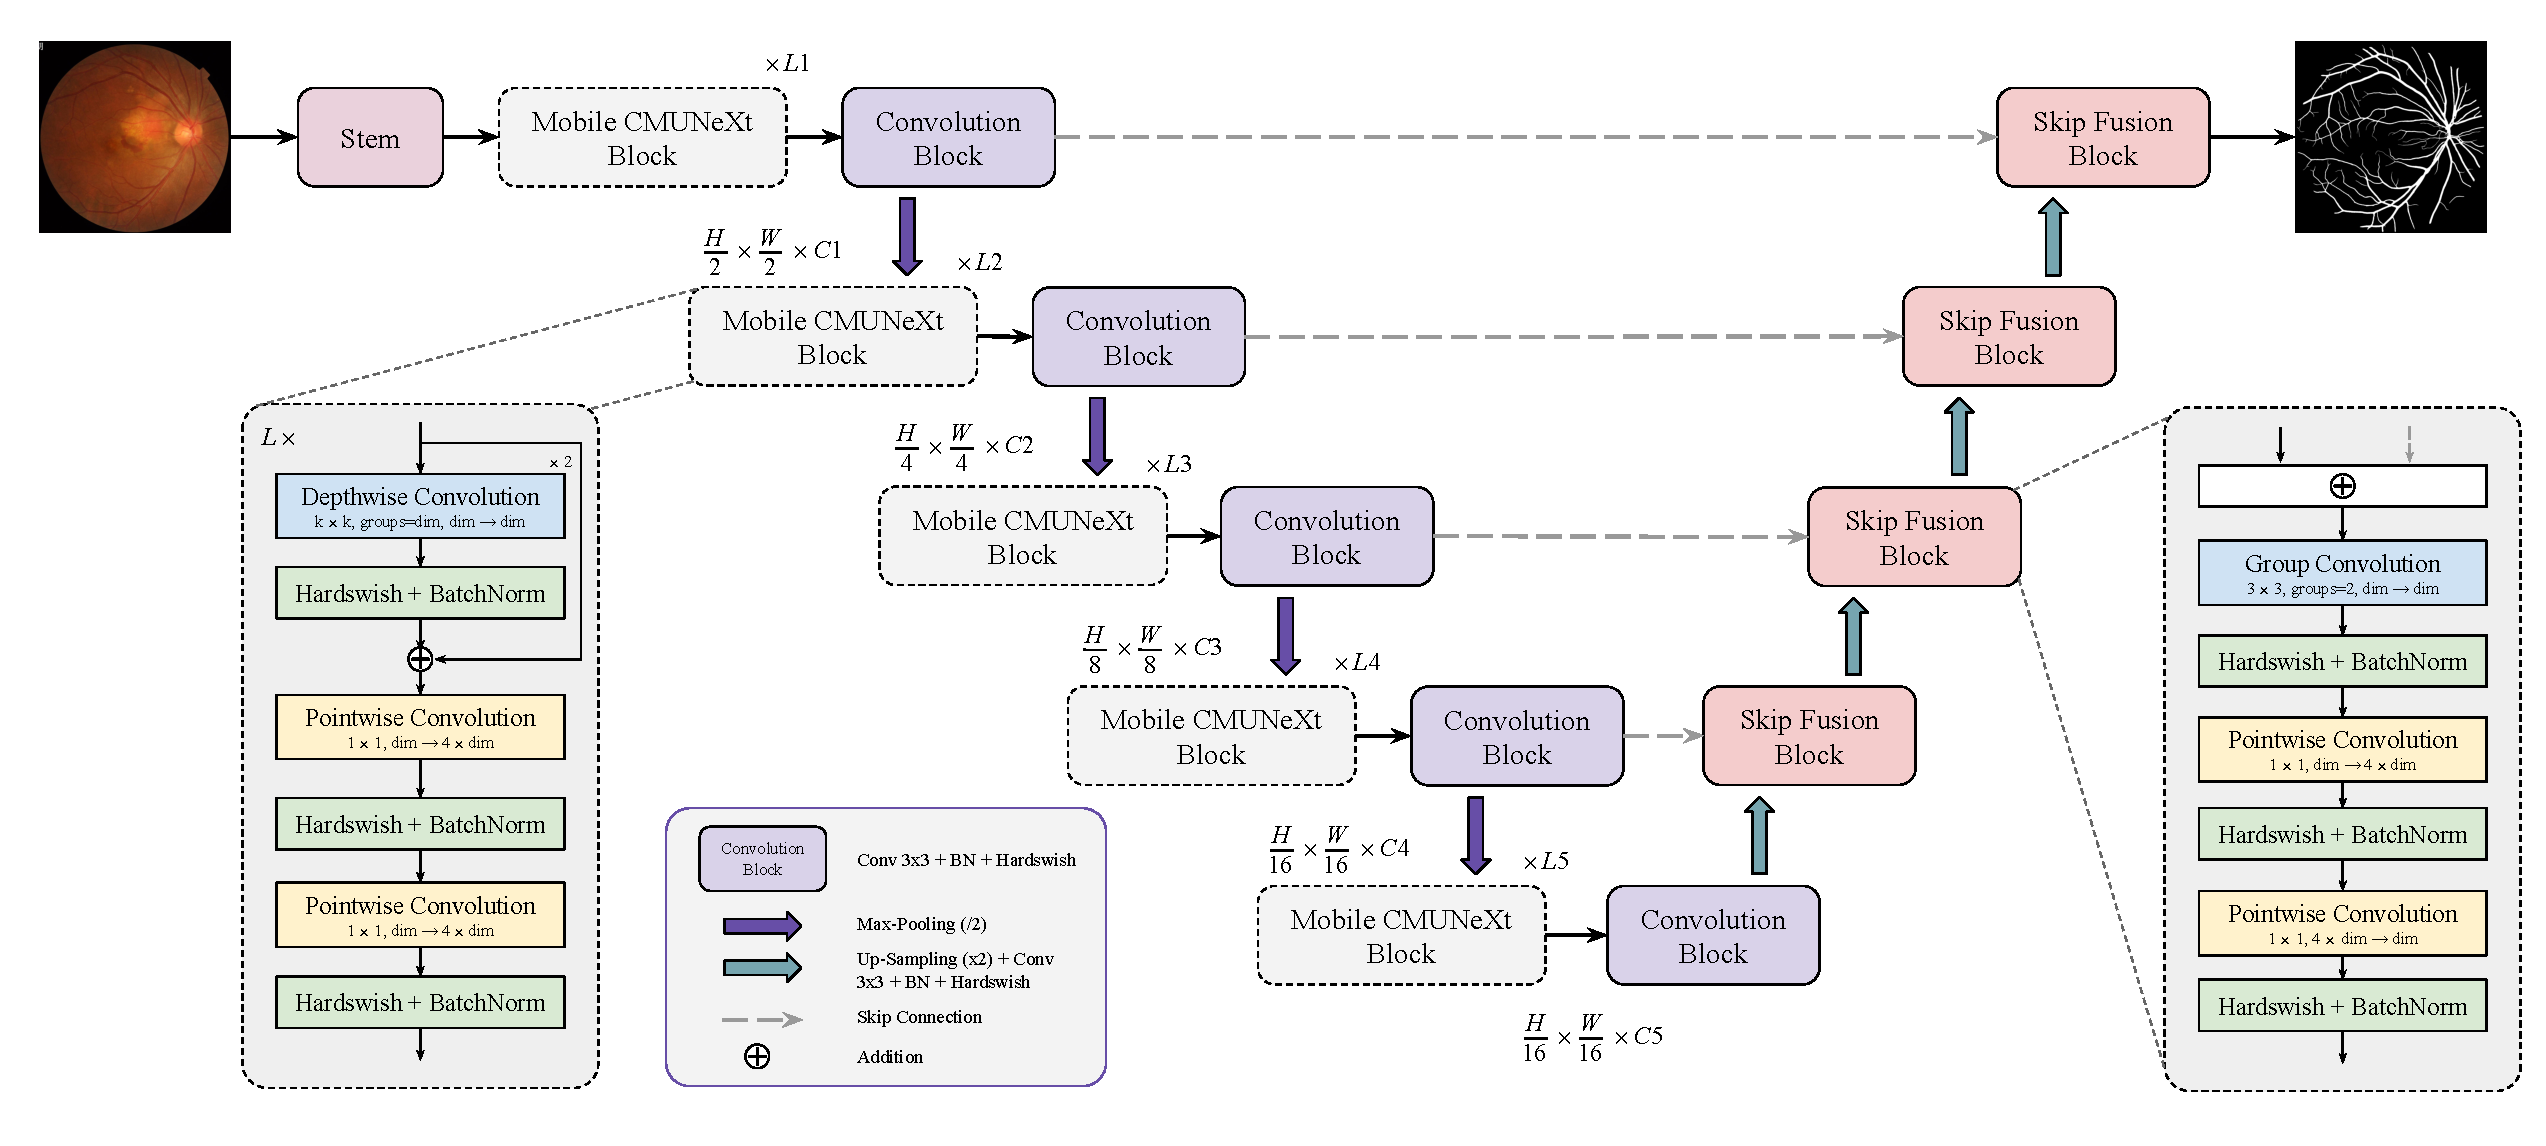
\includegraphics[width=\textwidth]{figures/Network Architecture.pdf}
    \caption{Overview Mobile-CMUNeXt}
    \label{fig:mobilecmunext-arch}
\end{figure*}


\subsection{Activation Function}
Another difference in the proposed network is the use of the Hardswish activation function, popularized in the MobileNetV3 \cite{koonce2021mobilenetv3}. This function tries to emulate the GELU activation function, used in the original network, but with a computationally less expensive. While GELU relies on the error function to approximate a smooth transition, Hardswish replaces it with a simple piecewise linear function. This makes Hardswish more efficient while still retaining non-linearity benefits similar to GELU. 

The Hardswish activation function is defined as:

\[
\text{Hardswish}(x) =
\begin{cases} 
0, & \text{if } x \leq -3, \\
x, & \text{if } x \geq +3, \\
x \cdot (x + 3) \cdot \frac{1}{6}, & \text{otherwise}.
\end{cases}
\]

In comparison, the GELU activation function is given by:

\[
\text{GELU}(x) = x \cdot \Phi(x)
\]

where \(\Phi(x)\) is the cumulative distribution function of the standard normal distribution.

Figure \ref{fig:activation_comparison} illustrates the comparison between the Hardswish and GELU activation functions. The blue curve represents the Hardswish function, while the dashed red curve represents the GELU function. As seen in the plot, Hardswish approximates the GELU function's smooth curve, but with a simpler piecewise linear form.

\begin{figure}[htbp]
    \centerline{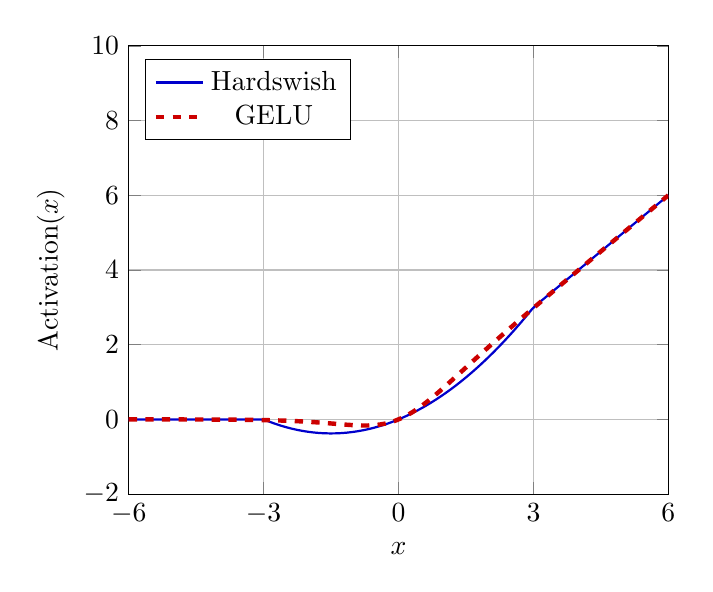
\begin{tikzpicture}
    \begin{axis}[
        grid=major,
        xlabel=$x$,
        ylabel=$\text{Activation}(x)$,
        legend pos=north west,
        xmin=-6,
        xmax=6,
        ymin=-2,
        ymax=10,
        xtick={-6,-3,...,6},
        ytick={-2,0,...,10},
    ]
        % Regular Hardswish
        \addplot[
            thick,
            color=blue!80!black,
            solid,
            samples=100,
            domain=-6:6
        ] {
            max(0,min(6,x+3)) * x / 6
        };
    
        % GELU Approximation
        \addplot[
            ultra thick,
            color=red!80!black,
            dashed,
            samples=100,
            domain=-6:6
        ] {
            x * (1 / (1 + exp(-1.702 * x)))
        };

        \legend{
            {Hardswish},
            {GELU}
        }
    \end{axis}
\end{tikzpicture}}
\caption{Comparison of Hardswish and GELU activation functions. Hardswish (blue solid line) and GELU (red dashed line)}
\label{fig:activation_comparison}
\end{figure}

Throughout the project, multiple activation functions were tested, namely: RELU, GELU, LeakyRELU and Harsdswish.
From all tested functions, the Hardswish activation function was chosen as it scales well with quantization (to be explained later in this document) and provides the best results.  

\subsection{Encoder}

\subsubsection{Stem}
The stem is designed to extract features from the original image at the top level, it is composed of a 2D Convolution layer with a kernel $3 \times 3$ , a stride of 1, and a padding of 1, followed by a 2D Batch Normalization layer and an inplace Hardswish Activation layer.

\subsubsection{Mobile-CMUNeXt Block}
Just like the original network this block is the most important component of the network and is characterized by the use of Depthwise Separable Convolutions. This is where most of the feature extraction occurs and therefore it is a crucial component in the network. It consists of two Depthwise 2D Convolution Layers connected sequentially with a variable kernel size of $k \times k$, group size of $dim$ dimension, and a padding of $k \div k$. This is followed by an expanding Pointwise 2D Convolution that transforms the feature map from $dim$ to $dim \times 4$, using a fixed kernel size of $1 \times 1$, a Hardswish activation function, and a 2D Batch Normalization layer. Next, a contracting Pointwise 2D Convolution that reduces the feature map from $dim \times 4$ to $dim$, again with a fixed kernel size of $1 \times 1$ and the same activation and normalization functions all connected sequentially. This block is repeated \textit{L} times, with each replication attempting to enhance the network feature extraction capacity, but at the cost of increasing the network parameters and size. 

\subsubsection{Downsampling}
The downsampling operation is performed using a 2D MaxPooling function, which helps reduce the spatial dimensions of the input while retaining important features. This is achieved with a fixed kernel size of $2 \times 2$ and a stride of $2$, meaning that the pooling operation will consider a $2 \times 2$ region at a time and move with a step of $2$ pixels in both horizontal and vertical directions. This effectively reduces the resolution of the feature map by half.


\subsection{Decoder}
\subsubsection{Skip Fusion}
The Skip Fusion block is used to fully fuse global semantic features from the encoder with up-sampled features from the decoder. It is composed of a group Convolution as the main technique. This convolution operation is split into two groups, performing "feature by feature" extraction separately on the encoder skipped features and the upsampled decoder features. The group convolution has a kernel size of $3 \times 3$, a stride of $1$, and padding of $1$. To combine the features effectively, two pointwise convolutions were added after the group convolution. 

Each convolution in the Skip Fusion block is followed by a Hardswish Activation function and a 2D Batch Normalization layer to help with stability and learning. The Skip Fusion block is defined as:
\begin{equation}
f_{concat}=Sum{
\left(
\begin{array}{l}
BN{\{}Conv2D(f_{\mathcal{E}}){\}}, \\
BN{\{}Conv2D(f_{\mathcal{D}}){\}}
\end{array} 
\right)
}
\end{equation}
\begin{equation}
f_{fusion}^{\prime}=BN\left(\sigma_1\left\{PointwiseConv2D\left(f_{concat}\right)\right\}\right)
\end{equation}
\begin{equation}
f_{fusion}=BN\left(\sigma_1\left\{PointwiseConv2D\left(f_{fusion}^{\prime}\right)\right\}\right)
\end{equation}

where $f_{\text{fusion}}$ is the final fused feature map, and $f_E$ and $f_D$ are the encoder and decoder features, respectively.

\subsubsection{Upsampling}
The upsampling block includes an upsampling layer, a convolutional layer, a batch normalization layer, and a Hardswish activation. Bilinear interpolation is used to upsample the feature maps by a factor of two. The convolutional layer uses a $3 \times 3$ kernel with a stride of 1 and padding of 1.

\section{Experiments}
In this section is provided a comprehensive evaluation of the proposed Mobile-CMUNeXt model against several state-of-the-art image segmentation networks, describing the datasets used in our experiments, followed by the training protocols, evaluation metrics, and a discussion of the various network models. It is also presented an ablation study and an analysis of quantization effects demonstrating the efficiency of Mobile-CMUNeXt.


\subsection{Datasets}

\paragraph{BUSI} The Breast UltraSound Images (BUSI) \cite{al2020dataset} public dataset collected from 600 female patients, includes 780 breast ultrasound images, covering 133 normal cases, 487 benign cases, and 210 malignant cases, each with corresponding ground truth labels. Only the benign and malignant cases from this dataset are utilized.

\paragraph{ISIC2016} The ISIC 2016 \cite{isic2016dataset} challenge dataset consists of dermoscopic images for skin lesion classification. It includes 900 training images and 379 test. Each image is provided with corresponding ground truth segmentation masks and diagnostic labels.

\paragraph{FIVES} Retinal vasculature provides an opportunity for direct observation of vessel morphology, which is linked to multiple clinical conditions. However, objective and quantitative interpretation of the retinal vasculature relies on precise vessel segmentation, which is time consuming and labor intensive. FIVES \cite{jin2022fives} dataset consists of 800 high-resolution multi-disease color fundus photographs with pixel-wise manual annotation. The annotation process was standardized through crowdsourcing of a group of medical experts. The quality of each image was evaluated, including illumination and color distortion, blur, and low contrast distortion, based on which the data splitting was conducted to make sure the balanced distribution of image features.

\subsection{Training}
All networks were trained in PyTorch using CUDA version 11.8 with the same conditions for a total of \textbf{300 epochs} and a \textbf{batch size} of 8. The \textbf{random seed} was set to 41 to ensure reproducibility of the results. All input images were resized to $256 \times 256$ pixels. The \textbf{Adam optimizer} with a \textbf{learning rate} of $1\times 10^{-3}$ and \textbf{weight decay of $1 \times 10^{-4}$} was used for optimization. The learning rate is adjusted using a \textbf{Cosine Annealing} scheduler with a maximum \textbf{T$_{\text{max}}$} of $1\times 10^{-3}$ and an \textbf{eta\_min} of $1.0 \times 10^{-5}$. All the experiments were conducted using a single NVIDIA GeForce RTX4080 GPU with the 535.183.01 driver version.


\subsubsection{Evaluation Metrics}
All models were evaluated using the following key metrics:

\begin{itemize}
    \item \textbf{IoU (Intersection over Union)}: IoU measures the overlap between the predicted segmentation mask and the ground truth mask. It is calculated as the ratio of the area of overlap to the area of union between the predicted and ground truth masks:

    \[
    \text{IoU} = \frac{|A \cap B|}{|A \cup B|}
    \]
    where \( A \) and \( B \) are the predicted and ground truth regions, respectively.

    \item \textbf{Dice}: The Dice coefficient is a metric for measuring the similarity between two sets. Ranges from 0 to 1 with 1 indicating perfect overlap. The Dice coefficient is defined as:

    \[
    \text{Dice} = \frac{2 |A_{\text{val}} \cap B_{\text{val}}|}{|A_{\text{val}}| + |B_{\text{val}}|}
    \]
    where \( A_{\text{val}} \) and \( B_{\text{val}} \) represent the predicted and ground truth regions on the validation set.

    \item \textbf{SE (Sensitivity)}: Sensitivity measures the ability of the model to correctly identify positive samples, like foreground objects in segmentation. It is calculated as the ratio of true positives to the sum of true positives and false negatives:

    \[
    \text{SE} = \frac{TP}{TP + FN}
    \]
    where \( TP \) is the number of true positives and \( FN \) is the number of false negatives.

    \item \textbf{PC (Precision)}: Precision measures the ability of the model to correctly predict positive samples out of all predicted positives. It is calculated as the ratio of true positives to the sum of true positives and false positives:

    \[
    \text{PC} = \frac{TP}{TP + FP}
    \]
    where \( TP \) is the number of true positives and \( FP \) is the number of false positives.

    \item \textbf{F1 Score}: The F1 score is the harmonic mean of precision and recall, providing a balanced measure of the model’s performance. It is useful when both precision and recall are important, especially in cases of imbalanced classes. The F1 score is defined as:

    \[
    F1 = 2 \cdot \frac{\text{Precision} \cdot \text{Recall}}{\text{Precision} + \text{Recall}}
    \]
    where \(\text{Precision}\) and \(\text{Recall}\) are defined as in the previous equations.

    \item \textbf{AAC (Average Accuracy per Class)}: The Average Accuracy per Class (AAC) measures the average accuracy for each class, calculated as the ratio of correct predictions for each class to the total number of samples for that class:

    \[
    \text{AAC} = \frac{1}{N} \sum_{i=1}^{N} \frac{TP_i}{TP_i + FN_i}
    \]
    where \( N \) is the number of classes, and \( TP_i \) and \( FN_i \) are the true positives and false negatives for class \( i \), respectively.

    \item \textbf{Loss}: The loss function \(\mathcal{L}\) quantifies the difference between the predicted output \(\hat{y}\) and the ground truth \(y\). It is calculated as a weighted combination of binary cross-entropy (BCE) and dice loss (Dice):
    \begin{equation}
        \mathcal{L} = 0.5 \cdot \text{BCE}(\hat{y}, y) + \text{Dice}(\hat{y}, y)
    \end{equation}

\end{itemize}



\subsubsection{Network Models}
For all experiments, multiple and diverse neural networks ranging from lightweight models to large models and transformer-based models were considered. Recently developed networks were also taken into consideration to compare the latest improvements in the field. Table~\ref{tab:networks} provides an overview of these networks grouped into UNet variant architectures, lightweight models, transformer-based models, and the proposed model.


\begin{table}[ht]
    \centerline{\begin{tabular}{|c|c|}
    \hline
    \textbf{Category} & \textbf{Network} \\
    \hline
    \multirow{4}{*}{U-Net Variants} & UNet \\
                                & UNetV2 \\
                                & UNet++ \\
                                & AttentionUNet \\ 
    \hline
    \multirow{6}{*}{Lightweight} & CMUNeXt \\
                                 & CFPNetM \\
                                 & UNeXt \\
                                 & GIVTED-Net \\
                                 & LUCF-Net \\
                                 & ULite \\
    \hline
    Transformer-based & TransUnet \\ 
    \hline
    \textbf{Proposed Network} & Mobile-CMUNeXt \\ 
    \hline
\end{tabular}}
\caption{Categorization of networks used in our experiments.}
\label{tab:networks}
\end{table}

\subsection{Mobile-CMUNeXt Model}
The \textbf{Mobile-CMUNeXt} builds upon the CMUNeXt family of architectures with optimizations to enhance feature extraction, reduce parameter count, and improve inference speed. The motivation behind our network comes from the need for a model that balances accuracy and efficiency, making it suitable for resource-constrained environments like FPGAs. Compared to the original model and its variants, Mobile-CMUNeXt has a significant reduction in the number of channels and block lengths but keeps the same large kernels as the CMUNeXt-S. Table~\ref{tab:variants} illustrates a comparison between different CMUNeXt variants and the proposed Mobile-CMUNeXt model.

\begin{table*}[t]
    \fittowidth{\begin{tabular}{>{\centering\arraybackslash}m{2.5cm}|ccccc|ccccc|ccccc}

\toprule[1.1pt]

\multirow{2}{*}[-0.5em]{Network} & \multicolumn{5}{c|}{Number of Channels} & \multicolumn{5}{c|}{Length of Blocks} & \multicolumn{5}{c}{Kernel Size}\\
\cmidrule{2-16}

\multicolumn{1}{c|}{}  & \textit{C}1 &  \textit{C}2 & \textit{C}3 & \textit{C}4 & \textit{C}5 & \textit{L}1 &  \textit{L}2 & \textit{L}3 & \textit{L}4 & \textit{L}5 & \textit{K}1 &  \textit{K}2 & \textit{K}3 & \textit{K}4 & \textit{K}5 \\

\midrule[0.7pt]

CMUNeXt-L 
& 32 &  64 & 128 & 256 & 512 
& 1 &  1 & 1 & 6 & 3 
& 3 &  3 & 7 & 7 & 7 \\

CMUNeXt 
& 16 & 32 & 128 & 160 & 256 
& 1 &  1 & 1 & 3 & 1 
& 3 &  3 & 7 & 7 & 7 \\

CMUNeXt-S  
& 8 & 16 & 32 & 64 & 128 
& 1 & 1 & 1 & 1 & 1 
& 3 & 3 & 7 & 7 & 9 \\

\midrule[0.7pt]

\textbf{CMUNeXt-XXS}
& 8 & 10 & 12 & 16 & 24 
& 3 & 1 & 1 & 2 & 3 
& 3 &  3 & 7 & 7 & 9 \\

\bottomrule[1.1pt]
\end{tabular}
}
    \caption{CMUNeXt variants and Mobile-CMUNeXt's custom configuration (CMUNeXt-XXS)} 
    \label{tab:variants}
\end{table*}


\subsection{Quantization}
As mentioned before, the final model will be quantized to reduce computational cost and improve inference speed in resource-constrained hardware, an FPGA in this work. Quantization was achieved using the  Brevitas 0.11.0 \cite{brevitas} framework which enables model quantization by applying custom quantization schemes to both weights and activations during the forward pass and providing custom PyTorch compatible modules. This technique allows for the reduction of the bit-width of the activations, the bias, and the weights leading to faster inference with lower memory requirements.

%\subsubsection{Quantized Hardswish}
The Quantized Hardswish activation function is implemented by modifying the standard Hardswish function to support quantization. The Brevitas' quantization tools were used to apply a custom bit-width to both the input and output of the activation function, enabling efficient processing. Additionally, the constant factor $\frac{1}{6}$ of the hardswish was approximated to $0.75$ to facilitate the quantization process and the division operation of the function.

\begin{figure}[htbp!]
    \centerline{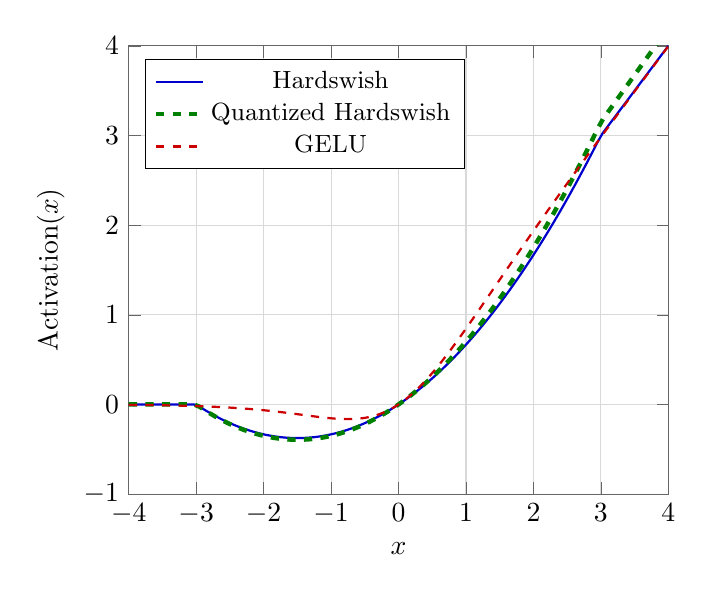
\begin{tikzpicture}
\begin{axis}[
    grid=major,
    xlabel=$x$,
    ylabel=$\text{Activation}(x)$,
    legend pos=north west,
    xmin=-4, xmax=4,
    ymin=-1, ymax=4,
    xtick={-4,-3,...,4},
    ytick={-1,0,...,4},
    legend style={font=\small},
    axis line style={gray!80!black},
    tick style={gray!80!black},
    grid style={gray!30},
]

    % Regular Hardswish
    \addplot[
        thick,
        color=blue!80!black,
        solid,
        samples=100,
        domain=-4:4
    ] {
        max(0,min(6,x+3)) * x / 6
    };

    % Quantized Hardswish
    \addplot[
        ultra thick,
        color=green!50!black,
        dashed,
        samples=100,
        domain=-4:4
    ] {
        max(0,min(6,x+3)) * x * 0.175
    };

    % GELU Approximation
    \addplot[
        thick,
        color=red!80!black,
        dashed,
        samples=100,
        domain=-4:4
    ] {
        x * (1 / (1 + exp(-1.702 * x)))
    };

    \legend{
        Hardswish,
        Quantized Hardswish,
        GELU
    }

\end{axis}
\end{tikzpicture}
}
\caption{Comparison of standard Hardswish (blue solid line) and Quantized Hardswish (red dashed line) activation functions. The quantized version uses a scaling factor of 0.175, resulting in reduced activation values while maintaining the same general shape as the original function.}
\label{fig:hardswish-comparison}
\end{figure}



\subsection{Results}
The training results can be found in Table~\ref{tab:results}. All metrics are reported with two decimal places. 

Given the results Mobile-CMUNeXt demonstrates an exceptional balance between efficiency and performance across all datasets. With only \textbf{0.04M parameters} and \textbf{0.47G MACs}, it is the lightest model in the benchmark while still maintaining competitive segmentation accuracy.  

Compared to the base CMUNeXt model (\textbf{3.14M parameters, 7.41G MACs}), Mobile-CMUNeXt achieves a \textbf{98.7\% reduction in parameters} and \textbf{93.6\% reduction in MACs} while maintaining comparable performance across ISIC2016, BUSI, and FIVES datasets.  

\begin{itemize}
    \item \textbf{ISIC2016:} Mobile-CMUNeXt achieves an \textbf{IoU of 84.94\%}, very close to CMUNeXt (84.99\%) and outperforming CMUNeXt-S (84.87\%). 

    \item \textbf{BUSI:} Mobile-CMUNeXt achieves \textbf{65.81\% IoU}, outperforming CMUNeXt-S (64.12\%) and coming close to CMUNeXt (65.84\%). It also performs competitively with CFPNetM (67.10\%), which has \textbf{19x more parameters}.  

    \item \textbf{FIVES:} Mobile-CMUNeXt achieves \textbf{75.00\% IoU}, surpassing CMUNeXt (68.77\%) and CMUNeXt-L (74.82\%) despite being \textbf{207x smaller}. The quantized version, Mobile-CMUNeXt-Quant, further improves to \textbf{77.44\% IoU}.  
\end{itemize}

Overall, Mobile-CMUNeXt proves to be an efficient alternative to the existing models, offering state-of-the-art segmentation performance while being lightweight and working for resource-constrained environments.  


\begin{table*}[htb]
    \fittowidth{\newcommand{\firstgroup}{3}  % First group column count (Networks, Params, MACS)
\newcommand{\metricgroup}{2}  % Columns per metric group (IoU, F1, AAC)
\newcommand{\totmetrics}{6}  % Total metrics columns (3 groups × metrics)
\newcommand{\metricstart}{4} % column where metrics start
\newcommand{\metricsend}{9} % column where metrics end

\begin{tabular}{ccc|cc|cc|cc}
\toprule[1.1pt]


\multirow{2}{*}[-0.5em]{\centering Network} &  
\multirow{2}{*}[-0.5em]{\centering MACS (G)$\downarrow$} &
\multirow{2}{*}[-0.5em]{\centering Params\ (M)$\downarrow$} &
\multicolumn{\metricgroup}{c|}{BUSI}  & 
\multicolumn{\metricgroup}{c|}{FIVES} & 
\multicolumn{\metricgroup}{c}{ISIC2016}
\\ 

\cmidrule{\metricstart-\metricsend}

\multicolumn{\firstgroup}{c|}{} % empty fist 3 columns 
& F1$\uparrow$ & IoU$\uparrow$
& F1$\uparrow$ & IoU$\uparrow$
& F1$\uparrow$ & IoU$\uparrow$
\\ 

\midrule[0.7pt]

AttentionUNet
& 66.63 & 34.88 	% MACS, PARAMS
& 74.53 & 61.9 	% BUSI (F1, iou)
& 82.08 & 69.75 	% FIVES2022 (F1, iou)
& 90.76 & 83.4 	% ISIC2016 (F1, iou)
\\

UNet
& 65.52 & 34.53 	% MACS, PARAMS
& 74.89 & 61.1 	% BUSI (F1, iou)
& 80.18 & 67.0 	% FIVES2022 (F1, iou)
& 90.59 & 83.0 	% ISIC2016 (F1, iou)
\\

UNet++
& 34.9 & 9.16 	% MACS, PARAMS
& 73.88 & 61.16 	% BUSI (F1, iou)
& \textbf{89.2} & \textbf{80.54} 	% FIVES2022 (F1, iou)
& 90.88 & 83.67 	% ISIC2016 (F1, iou)
\\

UNet\_V2
& 5.1 & 24.9 	% MACS, PARAMS
& 76.37 & 63.28 	% BUSI (F1, iou)
& 72.94 & 57.43 	% FIVES2022 (F1, iou)
& 90.94 & 83.73 	% ISIC2016 (F1, iou)
\\

\midrule[0.7pt]

TransUnet
& 32.23 & 105.32 	% MACS, PARAMS
& 77.81 & 65.2 	% BUSI (F1, iou)
& 87.85 & 78.37 	% FIVES2022 (F1, iou)
& 91.56 & 84.69 	% ISIC2016 (F1, iou)
\\

\midrule[0.7pt]

CFPNetM
& 3.47 & 0.76 	% MACS, PARAMS
& \textbf{79.76} & \textbf{67.1} 	% BUSI (F1, iou)
& \underline{88.3} & \underline{79.06} 	% FIVES2022 (F1, iou)
& 91.88 & 85.16 	% ISIC2016 (F1, iou)
\\

CMUNeXt
& 7.42 & 3.15 	% MACS, PARAMS
& 78.94 & 65.84 	% BUSI (F1, iou)
& 81.46 & 68.77 	% FIVES2022 (F1, iou)
& 91.79 & 85.0 	% ISIC2016 (F1, iou)
\\

GIVTED-Net
& \textbf{0.37} & \underline{0.19} 	% MACS, PARAMS
& 77.92 & 64.6 	% BUSI (F1, iou)
& 86.37 & 76.02 	% FIVES2022 (F1, iou)
& \textbf{92.34} & \textbf{85.91} 	% ISIC2016 (F1, iou)
\\

LUCF-Net
& 8.59 & 6.93 	% MACS, PARAMS
& \underline{79.1} & \underline{66.17} 	% BUSI (F1, iou)
& 76.51 & 62.03 	% FIVES2022 (F1, iou)
& \underline{92.04} & \underline{85.37} 	% ISIC2016 (F1, iou)
\\

ULite
& 0.76 & 0.88 	% MACS, PARAMS
& 78.93 & 66.11 	% BUSI (F1, iou)
& 77.58 & 63.44 	% FIVES2022 (F1, iou)
& 91.49 & 84.47 	% ISIC2016 (F1, iou)
\\

\midrule[0.7pt]

UNeXt
& 0.57 & 1.47 	% MACS, PARAMS
& 77.56 & 64.01 	% BUSI (F1, iou)
& 59.72 & 42.71 	% FIVES2022 (F1, iou)
& 91.32 & 84.18 	% ISIC2016 (F1, iou)
\\

\midrule[0.7pt]

\textbf{Mobile-CMUNeXt}
& \underline{0.47} & \textbf{0.04} 	% MACS, PARAMS
& 78.93 & 65.81 	% BUSI (F1, iou)
& 85.69 & 75.0 	% FIVES2022 (F1, iou)
& 91.75 & 84.94 	% ISIC2016 (F1, iou)
\\

\bottomrule[1.1pt]
\end{tabular}}
\caption{Results on Medical Datasets}
\label{tab:results}
\end{table*}


\subsubsection{Ablation Study}  
To analyze the impact of different components in the original network and understand its behavior to specific modifications a series of experiments known as ablation study was performed. Table~\ref{tab:ablation_results} contains the results of our experiments.


\begin{table*}[!htb]
    \fittowidth{\begin{tabular}{>{\centering\arraybackslash}m{3cm}ccc|ccc|cc|cc|cc}
\toprule[1.1pt]
\multirow{2}{*}[-0.5em]{\centering Network} & 
\multirow{2}{*}[-0.5em]{\centering Params (M)$\downarrow$} & 
\multirow{2}{*}[-0.5em]{\centering MACs (G)$\downarrow$} &
\multirow{2}{*}[-0.5em]{\centering Activation} &
\multicolumn{3}{c|}{Quantization} &
\multicolumn{2}{c|}{ISIC2016} & 
\multicolumn{2}{c|}{BUSI} & 
\multicolumn{2}{c}{FIVES} \\

\cmidrule{5-7} \cmidrule{8-13}
\multicolumn{4}{c|}{} & 
W & 
B & 
A & 
IoU$\uparrow$ & 
F1$\uparrow$ & 
IoU$\uparrow$ & 
F1$\uparrow$ & 
IoU$\uparrow$ & 
F1$\uparrow$ \\ 
\midrule[0.7pt]


U-Net 
& 34.52 & 65.52 & RELU
& - & - & -  
& 83.00 & 90.59     
& 61.10 & 74.89     
& 67.00 & 80.18 \\  

\midrule[0.7pt]

CMUNeXt-S
& 0.42 & 1.09 & GELU
& - & - & -
& 84.87 & 91.71 
& 64.12 & 77.39
& 75.24 & 85.85 \\

\midrule[0.7pt]

CMUNeXt-S + Kernels 3
& 0.42 & 1.08 & GELU
& - & - & -  
& 84.11 & 91.24 
& 59.40 & 73.43
& 72.73 & 84.20 \\ 

\midrule[0.7pt]

CMUNeXt-S + Add
& 0.32 & 0.79 & GELU
& - & - & -  
& 84.54 & 91.50 
& 63.81 & 77.08
& 64.81 & 78.60 \\ 

\midrule[0.7pt]

\textbf{CMUNeXt-XXS + Add}
& \textbf{0.04} & \underline{0.47} & Hardswish
& - & - & -  
& 84.94 & 91.75 
& 65.81 & 78.93
& 75.00 & 85.71 \\ 

\textbf{CMUNeXt-XXS + Add}  
& \textbf{0.04} & \underline{0.47} & RELU
& - & - & - 
& 85.46 & 92.08 
& 64.74 & 78.14 
& 75.40 & 85.96 \\ 

\textbf{CMUNeXt-XXS + Add}  
& \textbf{0.04} & \underline{0.47} & LeakyRELU
& - & - & - 
& 84.56 & 91.56 
& 65.11 & 78.26
& 77.12 & 87.70 \\ 


\midrule[0.7pt]

\textbf{CMUNeXt-XXS + Add + Quant}  
& \textbf{0.04} & \underline{0.47} & Hardswish
& 8 & 16 & 8 
& 84.45 & 91.43 
& 65.24 & 78.84 
& 77.44 & 87.26 \\ 

\textbf{CMUNeXt-XXS + Add + Quant}  
& \textbf{0.04} & \underline{0.47} & RELU
& 8 & 16 & 8
& 84.01 & 90.99 
& 65.21 & 76.49 
& 76.91 & 86.88 \\ 


\bottomrule[1.1pt]
\end{tabular}}
    \caption{Ablation Study. In the quantization column, (W)eight, (B)ias and (A)ctivation represent the amount of bits used for quantization or "-" if no quantization was used}
    \label{tab:ablation_results}
\end{table*}



\section{Work Plan}

\subsection{Work Developed}
In this section, the progress made in the development of Mobile-CMUNeXt is outlined, from research and dataset preparation to network training and quantization. The work has been divided into multiple phases, each addressing critical aspects of the project.

\subsubsection{Phase 1: Research and Setup}
The project began with a state-of-the-art research and identified the needed frameworks for this work. During this stage, the following steps were done:
\begin{itemize}
    \item A review on semantic segmentation, FPGA acceleration, and quantization techniques.
    \item Evaluation and selection of a deep learning model suited for medical segmentation.
    \item Set up the development environment.
\end{itemize}

Once the foundational research and setup were completed the focus shifted to reviewing and acquiring the data necessary for training the segmentation model.

\subsubsection{Phase 2: Network Development}
With the environment prepared, the next phase focused on model development and experimentation:
\begin{itemize}
    \item Collecting and preprocessing of medical imaging datasets.
    \item Training of multiple deep learning networks, including baseline architectures and CMUNeXt, to evaluate their performance.
    \item Vast experiments with CMUNeXt, identifying strengths and areas for optimization.
    \item Documentation of the progress and insights in a work report, marking the completion of the initial development phase.
\end{itemize}

Following successful experimentation with CMUNeXt efforts, the development of the lightweight model Mobile-CMUNeXt was addressed.

\subsubsection{Phase 3: Optimization}
After experimenting and establishing a strong model foundation, the focus turned to optimizing CMUNeXt for efficient hardware deployment:
\begin{itemize}
    \item Development of Mobile-CMUNeXt, incorporating architectural enhancements to reduce computational complexity.
    \item Model quantization to minimize memory footprint and enhance inference speed.
    \item Collection of preliminary experiments with bit quantization to explore further optimizations.
\end{itemize}

\subsection{Future Work}
The next phase of this project focuses on the hardware implementation of Mobile-CMUNeXt, ensuring its efficient deployment on an FPGA. The planned steps are as follows:

\begin{itemize}
    \item \textbf{Extract quantized model weights}: Convert and export the quantized network parameters.
    \item \textbf{Design hardware network}: Design the hardware architecture for the Mobile-CMUNeXt model on FPGA.
    \item \textbf{Choose a suited FPGA board}: Evaluate and select the most suitable FPGA.
    \item \textbf{Implement hardware design}: Translate the model into a hardware description language (HDL) and synthesize it for execution on the selected FPGA.
    \item \textbf{Final optimizations}: Perform enhancements such as latency reduction, memory bandwidth optimizations, and parallel processing enhancements.
    \item \textbf{Final implementation}: Deploy the fully optimized network on the FPGA and validate its real-time performance.
    \item \textbf{Record results}: Conduct benchmarking and performance evaluations, documenting accuracy, latency, and resource utilization metrics.
    \item \textbf{Thesis writing}: Write the thesis document.
\end{itemize}

These steps aim to complete the transition from a software-based AI model to a fully optimized hardware-accelerated solution.

\subsection{Risk Analysis} 
The development of Mobile-CMUNeXt presents several risks and challenges that must be considered to ensure successful deployment on an FPGA platform. These risks span multiple phases, from software-based model development to hardware implementation. Figure~\ref{fig:swot} assess these risks by illustrating a SWOT (Strengths, Weaknesses, Opportunities, and Threats) analysis that maps the completed work and future tasks to key areas of concern.

\vspace{0.5cm}
\begin{figure*}
    \centerline{\begin{tcolorbox}[colframe=black, colback=white, sharp corners, boxrule=1pt, width=\textwidth]
    \begin{center}
        {\Large \textbf{SWOT Analysis of Mobile-CMUNeXt}}
    \end{center}

    \begin{minipage}{0.48\textwidth}
        \textbf{Strengths}
        \begin{itemize}
            \item \textbf{Low computational complexity}: Achieved through lightweight model architecture and quantization.
            \item \textbf{Real-time inference with FPGAs}: Future FPGA implementation will ensure efficient execution.
            \item \textbf{Optimized quantization techniques}: Initial experiments have successfully reduced precision while maintaining accuracy.
            \item \textbf{Energy-efficient for edge devices}: The model is designed for resource-constrained environments, making it suitable for real-world medical applications.
        \end{itemize}
    \end{minipage}
    \hfill
    \begin{minipage}{0.48\textwidth}
        \textbf{Weaknesses}
        \begin{itemize}
            \item \textbf{FPGA-specific optimizations required}: Hardware-aware adjustments are necessary to maximize efficiency.
            \item \textbf{Limited support for high-precision tasks}: The quantization process may reduce segmentation accuracy for small or complex structures.
            \item \textbf{Trade-off between accuracy and efficiency}: A fine balance must be achieved to ensure that performance is not compromised by aggressive model compression.
        \end{itemize}
    \end{minipage}
    \vspace{0.5cm}
    
    \begin{minipage}{0.48\textwidth}
        \textbf{Opportunities}
        \begin{itemize}
            \item \textbf{Integration into low-power medical devices}: The lightweight nature of Mobile-CMUNeXt makes it ideal for embedded medical systems.
            \item \textbf{Expansion into real-time healthcare applications}: FPGA acceleration will enable deployment in time-sensitive medical workflows.
            \item \textbf{Potential for further model compression}: Additional techniques such as mixed-precision quantization and weight pruning could further optimize efficiency.
        \end{itemize}
    \end{minipage}
    \hfill
    \begin{minipage}{0.48\textwidth}
        \textbf{Threats}
        \begin{itemize}
            \item \textbf{Competition with GPU-based solutions}: FPGA implementations must match or exceed GPU performance to be widely adopted.
            \item \textbf{Hardware compatibility challenges}: Selecting and optimizing for a specific FPGA board may introduce limitations.
        \end{itemize}
    \end{minipage}
\end{tcolorbox}}
\caption{SWOT Analysis}
\label{fig:swot}
\end{figure*}

\bibliographystyle{IEEEtran}
\bibliography{bibliography.bib}


\vfill

\end{document}


